\section{Theory}
\label{sec:Theory}
Some theoretical concepts of quantum optics are necessary to understand the ways
in which Serge Haroche and David Wineland experimentally observed fundamental
quantum mechanical effects. This section aims to introduce the basic model of a
fully quantum mechanical description of atom-light interaction, the Jaynes-Cummings model, and
one of the most frequently appearing consequences of it, Rabi oscillations.

\subsection{Jaynes-Cummings Hamiltonian}
Both, Serge Haroche and David Wineland, investigated and made use of the
shifts in energy levels and relative phases of states that appear when a laser
shines in on an atom.  In
order to give a useful and complete description of the interaction of atoms with
light, one has to take into
account that the energy levels of the atom and of the photon field are
both quantized. The first ``fully quantized'' approach for the case of coherent light
in a cavity and a two level system was given by Edwin Jaynes and Fred Cummings
in 1963 \cite{jaynes1963comparison}. To describe the system (following
\cite{gerry2005introductory}) 
we introduce the total Hamiltonian, consisting of the Hamiltonian for the 
 quantized photon field for a single mode, the Hamiltonian of the two level
 system consisting of a ground state $\ket{g}$ and an excited state $\ket{e}$ and the
 interaction Hamiltonian
\begin{align}
  \label{eq:JCM_H_tot}
  {\hat {H}}={\hat {H}}_{{{\text{field}}}}+{\hat {H}}_{{{\text{atom}}}}+{\hat
  {H}}_{{{\text{int}}}},
\end{align}
where, neglecting the zero point energies of field and atom,
\begin{align}
  \label{eq:JCM_H_field}
  \hat{H}_{\text{field}} &= \hbar \omega_{\text{f}}\, \hat{a}^\dagger
   \hat{a}\\
  \label{eq:JCM_H_atom}
  \hat{H}_{\text{atom}} &= \frac{\hbar \omega_a}{2} \, \hat{\sigma_3} \\
  \label{eq:JCM_H_int}
  \hat{H}_{\text{int}} &= \hbar \omega_{\text{int}} \left( \hat{\sigma}_+ +
\hat{\sigma}_-\right)\left(\hat{a} + \hat{a}^\dagger\right).
\end{align}
Here $\hat{a}^\dagger$ and $\hat{a}$ are the creation and annihilation operators
that appear in the quantization of the electromagnetic field\footnote{To solve
the free field equation of the electromagnetic field one usually uses the Fourier ansatz
$$A^\mu(x) = \int \text{d}\tilde{k} \sum_{\lambda=0}^3 \left[ a_\lambda(\vec{k})
\epsilon^\mu_\lambda(k)\text{e}^{-ikx} +
a^\dagger_\lambda(\vec{k})\epsilon^\mu_\lambda(k)^* \text{e}^{+ikx}\right], $$
where $\lambda$ goes over all possible polarizations. When demanding that
$A^\mu$ and its conjugate field $\pi^\nu$ obey the canonical quantization
relation, the resulting commutator relations for $a_\lambda$ and
$a_\lambda^\dagger$ allow the interpretation as creation and annihilation
operators.}, the Pauli matrix $\hat{\sigma_3} = \ket{e}\bra{e} - \ket{g}\bra{g}$
acts as the inversion operator of the atom, and the associated Pauli
matrices $\hat{\sigma}_+ = \ket{e}\bra{g}$ and $\hat{\sigma}_- = \ket{g}\bra{e}$
project any state $\ket{g}$ ($\ket{e}$) to $\ket{e}$ ($\ket{g}$) respectively
and can thus be seen as atomic transition operators. It is now useful to look at
the time evolution of the terms in the total Hamiltonian \eqref{eq:JCM_H_tot}.
To do so we switch to the interaction picture, using the Hamiltonian without
interaction $\hat{H}_0 = \hat{H}_{\text{atom}} + \hat{H}_{\text{field}}$ to
describe the time evolution of the operators. For the  annihilation operator we
have 
\begin{align}
  \label{eq:a_time_ev}
  \hat{a}(t) &= e^{i\hat{H_0}t/\hbar}\, \hat{a}(0)\, e^{-i\hat{H_0}t/\hbar}
  \nonumber \\
  \intertext{using the Baker-Campbell-Hausdorff formula, we obtain}
  &= \hat{a}(0) + \frac{it}{\hbar}\left[\hat{H}_0, \hat{a}\right] +
  \frac{1}{2!}\left(\frac{it}{\hbar}\right)^2\left[\hat{H}_0, \left[\hat{H}_0,
  \hat{a}\right] \right] + \dots \nonumber
  \intertext{The first commutator is $\left[\hat{H}_0, \hat{a}\right] = -\hbar \omega_f
  \hat{a}$ as $\hat{a}$ commutes with $\hat{H}_{\text{atom}}$ and
  $\left[\hat{a}^\dagger, \hat{a}\right]=-1$. The nested commutators will thus only add higher orders of $\omega_f$. The
time evolution then becomes}
&= \hat{a}(0) \left(1 - it\omega_f + (it\omega_f)^2 + \dots  \right) \nonumber
\\
&= \hat{a}(0) e^{-i\omega_f t}.\,\footnotemark
\end{align}
\footnotetext{By looking at the preceding footnote
and considering that $kx$ is a scalar product of four-vectors but the
integration over $\text{d}\tilde{k}$ is only over the three spatial components,
we see that the time evolution behavior is already built-in in this ansatz.}Correspondingly we obtain for the other operators
\begin{align}
  \label{eq:ops_time_ev}
  \hat{a}^\dagger(t) &= \hat{a}^\dagger(0)e^{i\omega_ft}\\
  \hat{\sigma}_\pm(t) &= \hat{\sigma}_\pm(0)e^{\pm i\omega_a t}
\end{align}
and therefore the full interaction Hamiltonian becomes
\begin{align}
  \label{eq:H_int_time_ev}
  \hat{H}_{\text{int}}(t) = \hbar \omega_{\text{int}} \left( \hat{\sigma}_+ \hat{a}
  \, e^{i(\omega_a-\omega_f)t} \right& + \hat{\sigma}_+ \hat{a}^\dagger\,
    e^{i(\omega_a+\omega_f)t}\nonumber\\ & \left\quad + \hat{\sigma}_-\hat{a}\, e^{-i(\omega_a+\omega_f)t}
+ \hat{\sigma}_-\hat{a}^\dagger \, e^{-i(\omega_a-\omega_f)t}\right).
\end{align}
Assuming that the photon frequency $\omega_f$ is close to the transition
frequency of the atom $\omega_a$, i.e. $\left| \omega_a-\omega_f \right|
\ll \omega_a+\omega_f $, the rotating wave approximation can be applied. This
means that all terms in $\hat{H}_{\text{int}}$ that oscillate with
$\omega_a+\omega_f$ are
neglected. Doing this and transforming back to the Schrödinger picture leaves us
with the total Hamiltonian
\begin{align}
  \label{eq:H_tot_rot_wave}
  \hat{H}_{\text{tot}}= \hbar \omega_f \hat{a}^\dagger \hat{a} + \frac{\hbar\omega_a}{2}\hat{\sigma}_3
  + \hbar \omega_{\text{int}}\left( \hat{\sigma}_+\hat{a} +
  \hat{\sigma}_-\hat{a}^\dagger  \right).
\end{align}
The last two terms can be seen as processes in which the atom absorbs or emits
one photon from the field while respectively changing its internal energy state.

\subsection{Rabi Oscillations}
Having found a Hamiltonian that describes the interaction of an atom with light,
it is now interesting to investigate how this interaction influences the
dynamics of the system. The original states of atom and field will no longer be
eigenstates of the system and thus undergo a continuous oscillation, called Rabi
oscillation. Both Serge Haroche and David Wineland made experimental use of
this effect in order to prepare and manipulate states. To describe the dynamics
it is first useful to split the Hamiltonian in \eqref{eq:H_tot_rot_wave} into
two parts, namely
\begin{align}
  \label{eq:H_I_H_II}
  \hat{H}_I &= \hbar\omega_f\underbrace{\left( \hat{a}^\dagger\hat{a} +
  \ket{e}\bra{e}\right)}_{\text{excitation number }\hat{N}_e} + \hbar \left( \frac{\omega_a}{2} -
\omega_f)\right)\underbrace{\left(\ket{e}\bra{e} +
\ket{g}\bra{g}\right)}_{\text{e$^-$ number projector }\hat{P}_e} \\
\hat{H}_{II} &= -\hbar \underbrace{\left(\omega_a -
\omega_f\right)\ket{g}\bra{g}}_{\equiv\Delta} +
\hbar\omega_{\text{int}}\left( \hat{\sigma}_+\hat{a} +
  \hat{\sigma}_-\hat{a}^\dagger  \right).
\end{align}
The first part $\hat{H}_I$ commutes with $\hat{H}_{\text{tot}}$ thus it is
conserved over time and any interesting dynamics of the system are described by
the second part. Let us now consider a state
\begin{align}
  \label{eq:psi_t}
  \ket{\psi(t)} = C_1(t)\ket{e}\ket{n} + C_2(t)\ket{g}\ket{n+1} 
\end{align}
with initial conditions $C_1(0) = 1$ and $C_2(0)=0$. The time evolution is
described by the time dependent Schrödinger equation
$i\hbar\frac{\text{d}}{\text{d}t}\ket{\psi(t)}
= \hat{H}_{II}\ket{\psi(t)}$. In the resonant case ($\Delta=0$) this can be
exactly solved and yields
\begin{align}
  \label{eq:psi_t_solution}
  C_1(t) &= \cos\left(\omega_{\text{int}}\sqrt{n+1}\,t\right) \\
  C_2(t) &= -i\sin\left(\omega_\text{int} \sqrt{n+1} \,t\right)
\end{align}

We see that the state of a two level system can be manipulated by sending in coherent
  light, a technique that is crucial for many quantum optics experiments. In this 
context a nomenclature for pulses is established, describing to what extent the
light interacts with the atom. A pulse of light is called ``$ r\pi$-pulse'' ($r\in \mathbb{R}$)
if it interacts with an atom such that
\begin{align}
  \label{eq:r_pulse}
  \omega_{\text{int}}\sqrt{n+1}\, t = \frac{r \pi}{2}.
\end{align}
A commonly used type of pulse is for example the $\pi/2$-pulse that takes e.g. a
pure state $\ket{e}\ket{n}$ to a superposition
state $\frac{1}{\sqrt{2}}\left(\ket{e}\ket{n}-i\ket{g}\ket{n+1}\right)$. In the basis spanned by $\left\lbrace
\ket{e}\ket{n}, \ket{g}\ket{n+1}\right\rbrace$ a $\pi/2$-pulse can be
represented in matrix form as
\begin{align}
  \label{eq:pi_half_matrix}
U(\pi/2) = \frac{1}{\sqrt{2}}  
\begin{pmatrix*}[r] 
      1 & -i \\
      -i & 1
    \end{pmatrix*}.
\end{align}
The repeated action of a $\pi/2$-pulse on a two level system is shown
graphically in Fig.~\ref{fig:rabi_cycle_rep}. It should be noted that starting
from $\ket{e}\ket{n}$ and performing a full Rabi cycle will introduce a global
phase of $-1$ to the system. However this phase is not of physical importance
when the two level system is closed and only measurable in comparison to a
reference system.\footnote{$\braket{e|\hat{O}|e} = \braket{e|(-1)\hat{O}(-1)|e}$
for any observable $\hat{O}$.}
\begin{figure}[h]
  \centering
  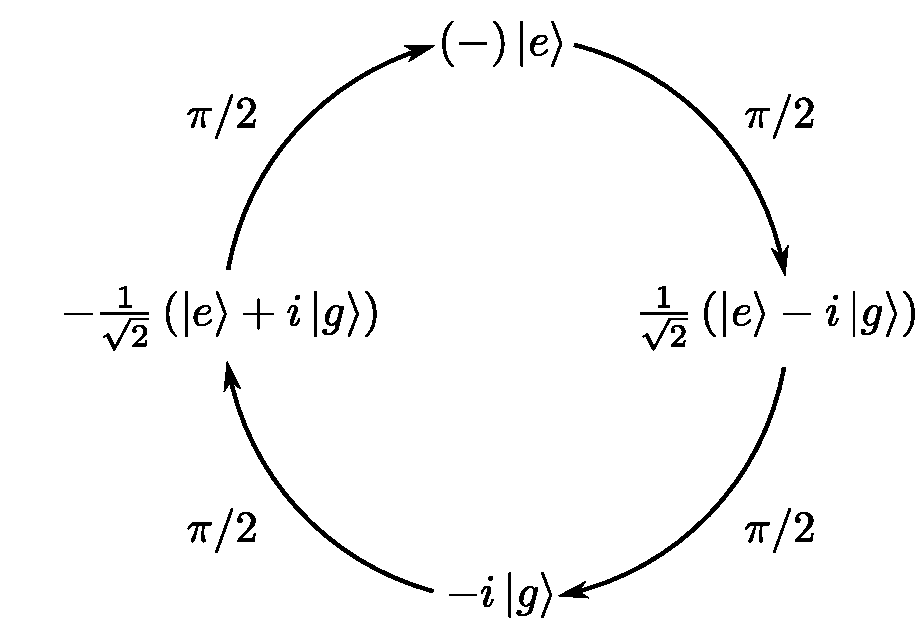
\includegraphics[width=.5\linewidth]{rabi_cycle_rep.pdf}
  \caption{Graphic representation of the action of a $\pi/2$-pulse on the state
    of a two level system. The photon number states (e.g. as in $\ket{e}\ket{n}$)
    are not shown explicitly. The $(-)$ in front of the excited state indicates
  the change of the total phase after one full cycle, which is of importance
only if there is another state to which it should be compared in measurement.}
  \label{fig:rabi_cycle_rep}
\end{figure}

\subsection{Dressed States}
\label{sec:DressedStates}
Description of the dynamics of a two level system in the
off-resonant case requires diagonalization of the Hamiltonian
\eqref{eq:H_tot_rot_wave}. The resulting eigenstates are called ``dressed
states'', a wording that suggests that they are atom states ``dressed in light'' in contrast
to the ``bare'' states of the atom without a light field. Using again the basis
$\left\lbrace \ket{e}\ket{n}, \ket{g}\ket{n+1}\right\rbrace$ we can represent
\eqref{eq:H_tot_rot_wave} as
\begin{align}
  \label{eq:H_tot_matrix}
  \hat{H}_{\text{tot}} = 
  \renewcommand*{\arraystretch}{2}
  \begin{pmatrix*}[c]
    n\omega_f + \frac{1}{2} \hbar\omega_a & \hbar\omega_{\text{int}} \sqrt{n+1}\\
    \hbar\omega_{\text{int}} \sqrt{n+1}\quad & (n+1)\omega_f - \frac{1}{2}\omega_a
  \end{pmatrix*}
\end{align}
and diagonalize it. From this we obtain the eigenenergies 
\begin{align}
  \label{eq:eigenergies}
  E_\pm = \hbar\omega_f\left(n+\frac{1}{2}\right) \pm \hbar\Omega_n(\Delta)
\end{align}
with the off-resonant Rabi frequency
\begin{align}
  \label{eq:Omega_n}
  \Omega_n(\Delta) = \sqrt{\Delta^2 + 4 \omega_{\text{int}}^2(n+1)}.
\end{align}
The eigenenergies of the new eigenstates depend on the detuning of the light
with respect to the atom transition. This shift in the energy levels is often
referred to as the ``AC-Stark-shift''.
The corresponding eigenstates in the given basis are
\begin{align}
  \label{eq:eigenstates}
  \ket{n,+} &=  \cos(\Phi_n/2)\ket{e}\ket{n} +  \sin(\Phi_n/2) \ket{g}\ket{n+1}\\ 
  \ket{n,-} &=  -\sin(\Phi_n/2)\ket{e}\ket{n} +  \cos(\Phi_n/2) \ket{g}\ket{n+1} 
\end{align}
where the angle $\Phi_n$ is given by
\begin{align}
  \label{eq:phi_n}
  \Phi_n = \tan^{-1}\left( \frac{2\omega_{\text{int}}\sqrt{n+1}}{\Delta} \right)
\end{align}
which converges towards $\pi/2$ for $\Delta\rightarrow 0$. The dressed states
are now useful for many applications in the field of quantum optics. Given a
prepared state of a two level atom, one can determine the interaction of the
atom with (not necessarily resonant) incident light by expressing the initial
state in terms of the dressed states. As the dressed states are eigenstates of
the total Hamiltonian their time evolution is trivial under application of the
time evolution operator. In this way the dynamics can be calculated in the
dressed states basis and afterwards (if needed) transformed back to the initial
basis.

\subsection{Far Off Resonance Case}
The full Jaynes-Cummings Hamiltonian \eqref{eq:JCM_H_tot} without the rotating
wave approximation can also be treated for the far off-resonant case
$\Delta\gg\omega_a$. Interaction is in this case ruled by the effective
Hamiltonian 
\begin{align}
  \label{eq:H_eff}
  \hat{H}_{\text{eff}} = \hbar \chi \left[\hat{\sigma}_+\hat{\sigma_-} +
  \hat{a}^\dagger \hat{a}\sigma_3 \right],
\end{align}
where $\chi$ depends on the photon number $n$ and the detuning $\Delta$
\cite{gerry2005introductory}. Under this Hamiltonian a state
\begin{align}
  \label{eq:psi_evol_0}
  \ket{\Psi(0)} = \frac{1}{\sqrt{2}} \left(\ket{e}\ket{n} +
  \ket{g}\ket{n}\right)
\end{align}
will evolve according to 
\begin{align}
  \label{eq:psi_evol_t}
  \ket{\Psi(t)} = \frac{1}{\sqrt{2}} \left( \ket{e}\ket{n} + e^{-i\,\chi
  (\Delta,n)t} \ket{g}\ket{n}\right),
\end{align}
a time evolution that Serge Haroche used to non-destructively detect single
photons (see Sec.~\ref{sec:QND}).
